\section{Auswertung und Diskussion}
\label{sec:Auswertung}

\subsection*{Bestrahlungsplan für das PTV1}

Die Dosisverteilung des ersten Bestrahlungsplans sind in den Abbildungen \ref{abb:Z}, \ref{abb:Y} und \ref{abb:X}
dargestellt. Dabei handelt es sich um die transversale, frontale und sagittale Ansicht des Kopfes.
Anhand der Isodosenlinien ist zu erkennen, dass das Ziel, das gesamte PTV mit der
$95\%$ Isodosenlinie zu umschließen, nicht erreicht werden konnte. Anhand der sagittalen Ansicht ist
zu erkennen, dass vor allem im dem Bereich des PTVs, der unmittelbar hinter den Augen liegt, nicht die gewünschte
Dosis erreicht werden konnte. Das kommt daher, da die Augenlinsen ein Risikoorgan sind und aus diesem Grund geschützt werden müssen.
Da innerhalb des PTVs nicht die gewünschte Dosisverteilung erreicht werden kann, liegt die minimale relative Dosis bei $63,6\%$.
Des weiteren ist zu erkennen, dass die maximale relative Dosis $112,3\%$ zum einen außerhalb des PTV deponiert werden und auch oberhalb der erlabten
maximalen Dosis von $107\%$ liegt \cite{ICRU}. Die maximale Dosis liegt außerhalb des PTVs, da die Photonenstrahlung zunächst den Schädelknochen
durchdringen muss, bevor es zu dem PTV gelangt. Durch die hohe Dichte des Schädels, wird dort auch eine hohe Dosis deponiert.


\begin{figure}[H]
  \centering
  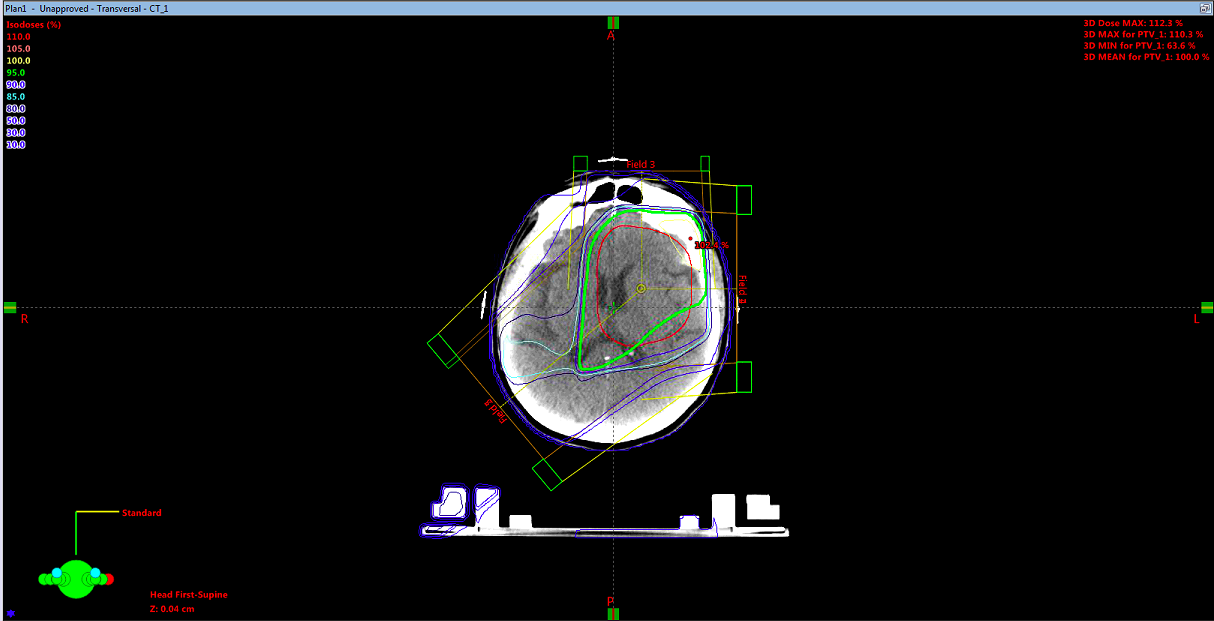
\includegraphics[width=\textwidth]{Bilder/Teilhirn1_Z.png}
  \caption{Darstellung der Dosisverteilung im Kopf in Transversalansicht.}
  \label{abb:Z}
\end{figure}

\begin{figure}[H]
  \centering
  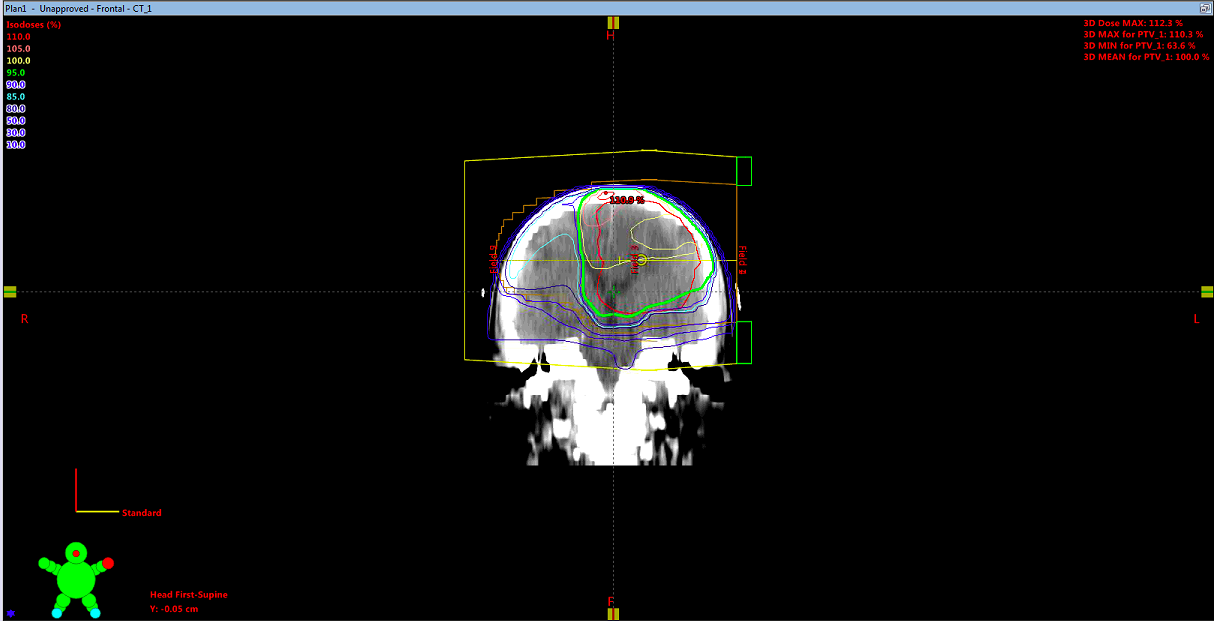
\includegraphics[width=\textwidth]{Bilder/Teilhirn1_Y.png}
  \caption{Darstellung der Dosisverteilung im Kopf in Frontalansicht.}
  \label{abb:Y}
\end{figure}

\begin{figure}[H]
  \centering
  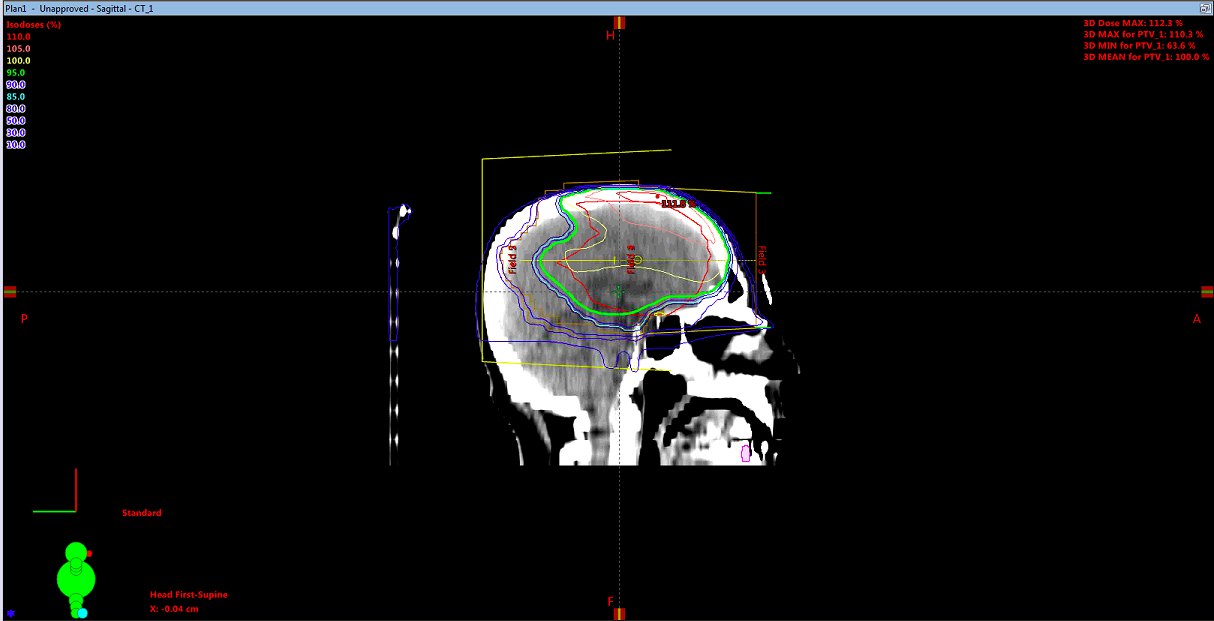
\includegraphics[width=\textwidth]{Bilder/Teilhirn1_X.png}
  \caption{Darstellung der Dosisverteilung im Kopf in Sagittalansicht.}
  \label{abb:X}
\end{figure}

Das zugehörige DVH ist in der Abbildung \ref{abb:DVH} gezeigt. Anhand des DVHs für das PTV1 ist zu erkennen, dass noch ein Teil des PTVs
eine relative Dosis von $95\%$ erhält. Noch etwa $95\%$ des PTVs erhält eine relative Dosis von $95\%$. Anhand dieser Kurve ist außerdem
zu erkennen, dass die maximale relative Dosis im PTV $110,3\%$ ist, allerdings nur ein sehr kleiner Teil des PTVs diese hohe Dosis erhält.
Mit der DVH Kurve des gesamten Schädels ist auch zu erkennen, dass nur ein sehr kleiner Teil eine relative Dosis von mehr als $107\%$ erhält.
Generell ist mit dieser Kurve zu sehen, dass in einem großen Teil des Kopfes eine hohe Dosis deponiert wird. Das kommt daher, dass das PTV bei dieser
Bestrahlung sehr groß ist.


\begin{figure}[H]
  \centering
  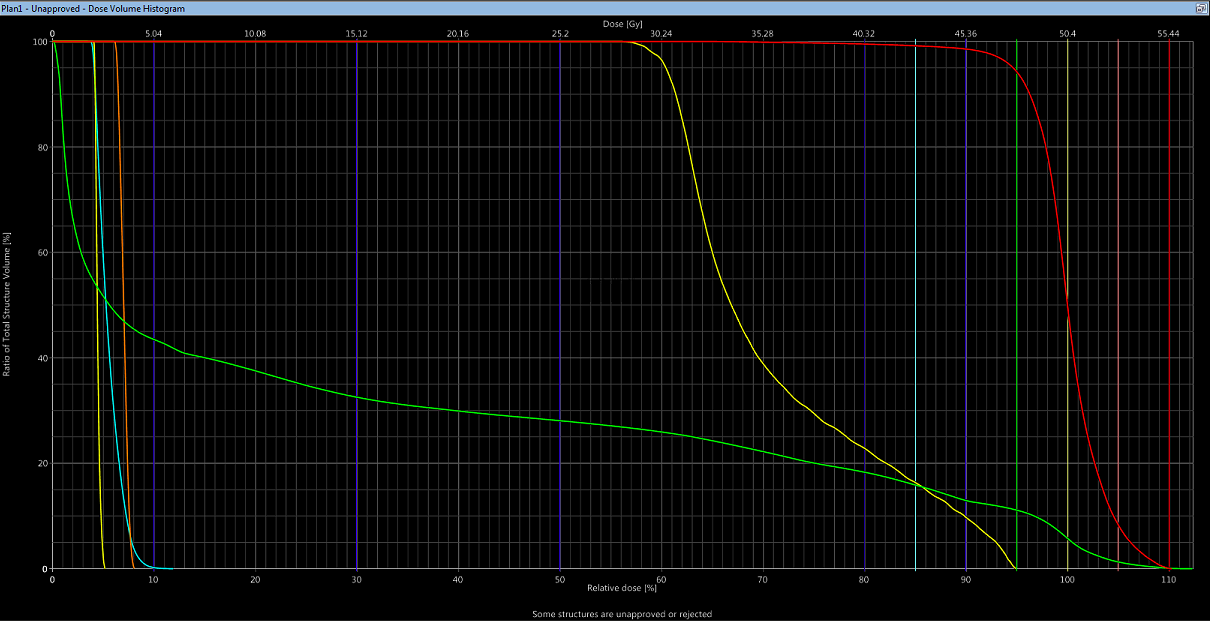
\includegraphics[width=\textwidth]{Bilder/Teilhirn1_DVH.png}
  \caption{Dosis-Volumen-Histogramm für das PTV1 in rot und den gesamten Schädel in grün. Außerdem ist das DVH für das Chiasma in gelb, für die linke Linse in orange, für die rechte Linse in gelb und für das rechte Auge in hellblau dargestellt.}
  \label{abb:DVH}
\end{figure}

Mit dem DVH Kurven der Risikoorgane wird außerdem überprüft ob die Organdosisgrenzwerte eingehalten werden.
Anhand der Kurven der Augenlinsen ist zu erkennen, dass in der linken Linse etwas mehr Dosis deponiert wird
als in der rechten Linse. Allerdings sind die maximalen relativen Dosen $8,1\%$ und $5,2\%$ was eine absolute Dosis von
$\SI{4.08}{\gray}$ und $\SI{2.62}{\gray}$ ergibt. Diese Werte liegen unterhalb von dem Organdosisgrenzwert
$\SI{5}{\gray}$ \cite{grenz}. Nach dem zweiten Bestrahlungsplan muss allerdings die gesamte Dosis der Augenlinsen noch betrachtet werden.
Das Chiasma konnte bei diesem Bestrahlungsplan nicht geschont werden. Die maximale relative Dosis die das Chiasma absorbiert ist
$94,9\%$, also eine absolute Dosis von $\SI{47.83}{\gray}$. Noch liegt diese Dosis unterhalb des Grenzwertes von
$\SI{54}{\gray}$, in dem zweiten Bestrahlungsplan muss das Chiasma allerdings besser geschont werden.
Anhand der DVH Kurve des rechten Auges ist zu erkennen, dass in den gesamten Augen nicht viel Dosis deponiert wird.


\subsection*{Bestrahlungsplan für das PTV2}

Die Dosisverteilung des zweiten Bestrahlungsplans ist in verschiedenen Ansichten in den
Abbildungen \ref{abb:Z2}, \ref{abb:Y2} und \ref{abb:X2} gezeigt. Anhand der Dosisverteilung ist
zu erkennen, dass im Gegensatz zu dem ersten Bestrahlungsplan, es in diesem Fall besser gelungen
ist das gesamte PTV2 mit der $95\%$ Isodosenlinie zu umschließen. An einigen Stellen ist dies allerdings auch in
diesem Fall nicht gelungen. Auch in bei diesem Bestrahlungsplan liegt die maximale relative Dosis $108,9\%$ außerhalb des
PTVs. Diese maximale Dosis wird in den Schädelknochen deponiert, da das PTV teilweise sehr nah an dem Schädelknochen liegt und dort durch die
große Dichte eine hohe Dosis absorbiert wird. Die minimale relative Dosis in dem PTV liegt bei $90,9\%$ und liegt nur knapp unterhalb der gewünschten
$95\%$, was auf eine gute Dosisverteilung in dem PTV schließen lässt.


\begin{figure}[H]
  \centering
  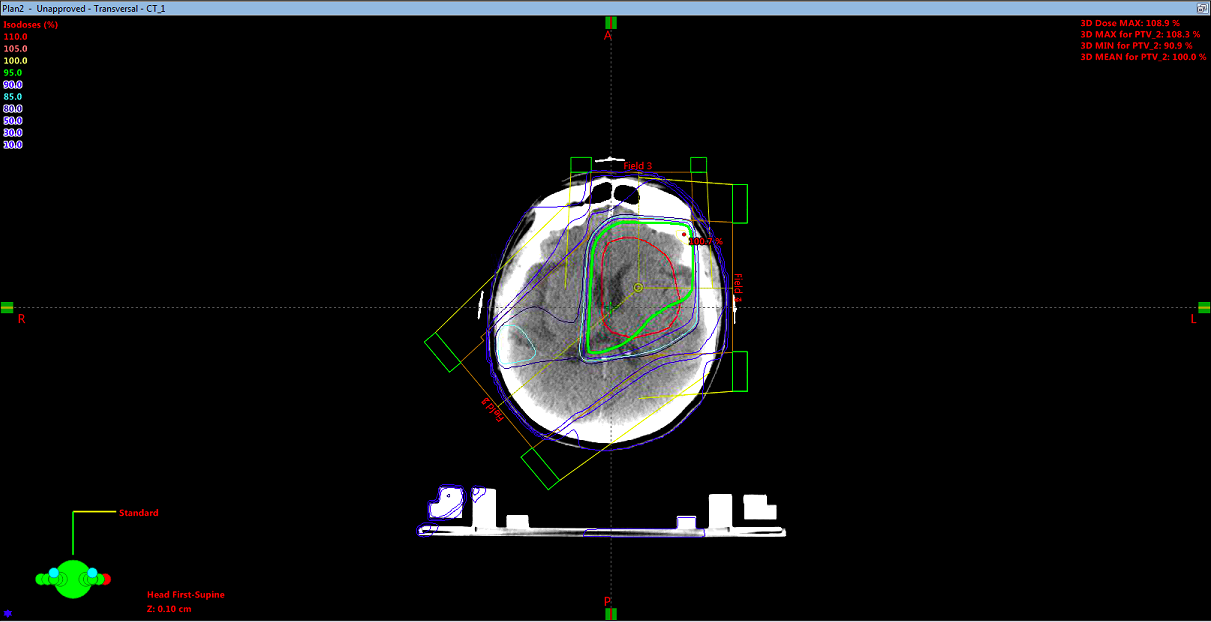
\includegraphics[width=\textwidth]{Bilder/Teilhirn2_Z.png}
  \caption{Darstellung der Dosisverteilung im Kopf in Transversalansicht.}
  \label{abb:Z2}
\end{figure}

\begin{figure}[H]
  \centering
  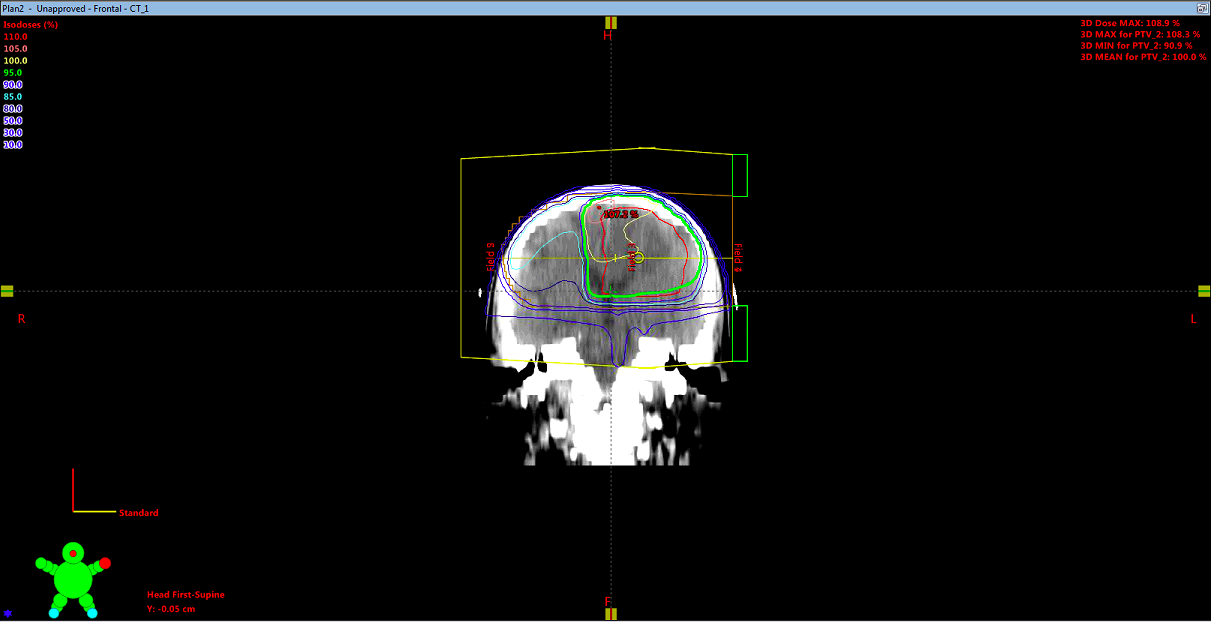
\includegraphics[width=\textwidth]{Bilder/Teilhirn2_Y.png}
  \caption{Darstellung der Dosisverteilung im Kopf in Frontalansicht.}
  \label{abb:Y2}
\end{figure}

\begin{figure}[H]
  \centering
  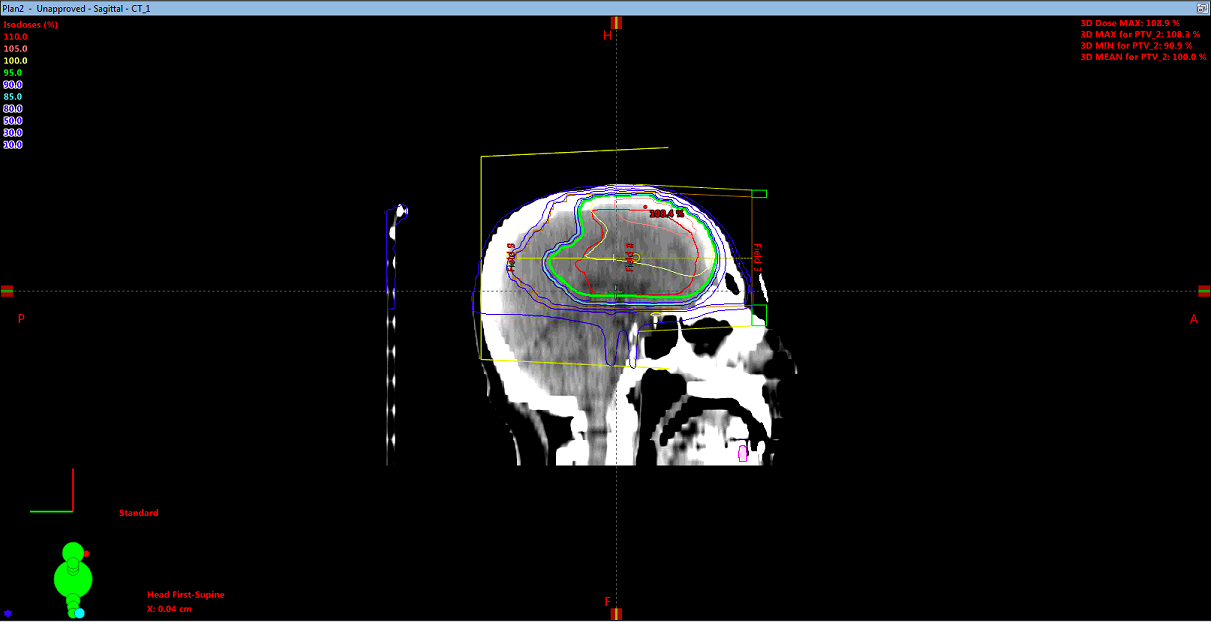
\includegraphics[width=\textwidth]{Bilder/Teilhirn2_X.png}
  \caption{Darstellung der Dosisverteilung im Kopf in Sagittalansicht.}
  \label{abb:X2}
\end{figure}

Auch für diesen Plan wird ein DVH erstellt um die Dosisverteilung besser beurteilen zu können.
Dieses DVH ist in der Abbildung \ref{abb:DVH2} gezeigt. Anhand des DVHs für das PTV ist zu erkennen, dass
etwa $97\%$ des PTVs eine relative Dosis von $95\%$ erhält. Die maximale Dosis innerhalb des PTVs liegt bei $108,3\%$, was über der erlaubten
maximalen Dosis von $107\%$ liegt. Es ist allerdings auch zu erkennen, dass sowohl in dem PTV, als auch in dem gesamten Schädel nur ein sehr kleiner
Teil eine relative Dosis von über $107\%$ erhält. Es sind außerdem wieder die DVHs der Risikoorgane dargestellt.
Anhand der Kurve für das Chiasma ist zu erkennen, dass es bei diesem Bestrahlungsplan gut geschont werden konnte und nur eine relative maximale
Dosis von $24,2\%$ erhält. Auch bei diesem Plan erhält die linke Augenlinse eine etwas größere Dosis als die rechte Augenlinse. Die maximalen Dosen
der Augenlinsen sind $7\%$ und $4\%$.

\begin{figure}[H]
  \centering
  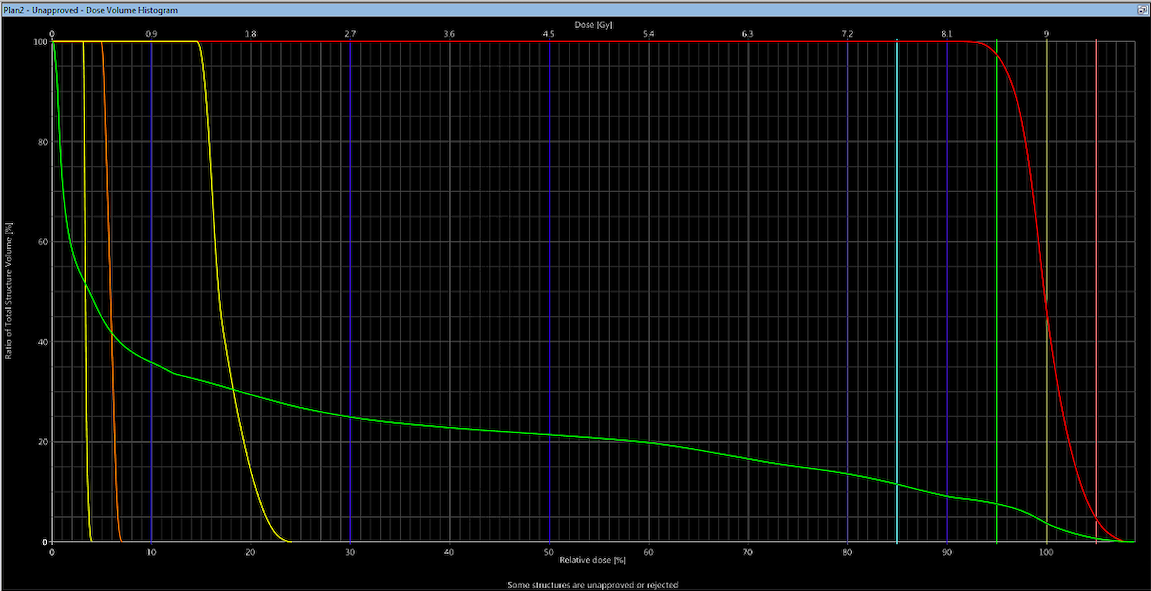
\includegraphics[width=\textwidth]{Bilder/Teilhirn2_DVH.png}
  \caption{Dosis-Volumen-Histogramm für das PTV2 in rot und den gesamten Schädel in grün. Außerdem ist das DVH für das Chiasma in gelb, für die linke Linse in orange und für die rechte Linse in gelb.}
  \label{abb:DVH2}
\end{figure}


\subsubsection*{Summe der Bestrahlungspläne}

In der Abbildung \ref{abb:DVHsum} ist das DVH der Summe der beiden Bestrahlungspläne dargestellt.
Bei diesem DVH ist auf der x-Achse die absolute Dosis angegeben. Dieses DVH ist gezeigt um zu überprüfen ob
die Organdosisgrenzwerte für die Augenlinsen und das Chiasma eingehalten worden sind.
Anhand der Kurven ist zu erkennen, dass die gesamte maximale Dosis der Augenlinsen $\SI{2.986}{\gray}$ und $\SI{4.722}{\gray}$ beträgt.
Beide Werte liegen unterhalb der Grenzwerte. Das Chiasma erhält eine gesamte maximale Dosis von $\SI{49.479}{\gray}$. Auch diese Dosis liegt unterhalb
des Grenzwertes von $\SI{54}{\gray}$ \cite{grenz}.

\begin{figure}[H]
  \centering
  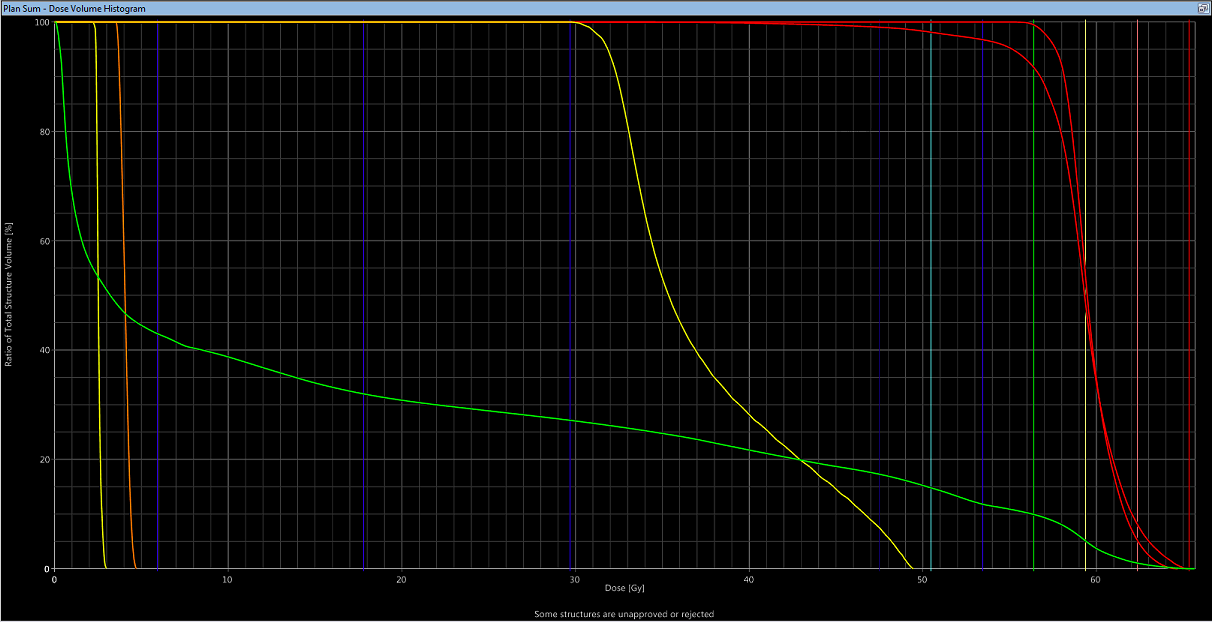
\includegraphics[width=\textwidth]{Bilder/Teilhirn_vergleich2.png}
  \caption{Dosis-Volumen-Histogramm für die Summe der beiden Bestrahlungspläne. Für das PTV1 und PTV2 in rot und den gesamten Schädel in grün. Außerdem ist das DVH für das Chiasma in gelb, für die linke Linse in orange und für die rechte Linse in gelb.}
  \label{abb:DVHsum}
\end{figure}


Insgesamt wurde durch die Verwendung von fünf Feldern gewährleistet, dass die
beiden Zielvolumina im ausreichenden Maße mit der $95\%$ Isodosenlinie umschlossen wurden.
Durch die Verwendung von MLCs ist erreicht worden, dass die Organdosisgrenzwerte für
die Augenlinsen und das Chiasma nicht überschritten werden.
